\documentclass{article}
\renewcommand{\familydefault}{\sfdefault}
\usepackage[a4paper, total={6in, 8in}]{geometry}
\usepackage{array}
\usepackage{amssymb}
\usepackage[version=4]{mhchem}
\usepackage{chemarr}
\usepackage{mathtools}
\usepackage{graphicx}
\graphicspath{ {./images/} }

\title{Ionic Equilibria}
\date{2021-05-05}
\author{Jeh}

\begin{document}
\maketitle
\pagenumbering{arabic}
   \section{One Mark Questions}
   \subsection{Why cations are Lewis acids?}
   Cations are electron-deficient species and can accept an electron pair.
   Hence, cations are Lewis acids.

   \subsection{Why is KCl solution neutral to litmus?}
   KCl, being salt of a strong acid(HCl) and a strong base(KOH), does not
   undergo hydrolysis. Hence, the KCl solution is neutral to litmus.

   \subsection{How are basic buffer solutions prepared?}
   Basic buffer solutions are prepared by mixing aqueous solutions of a weak
   base and its salt with strong acid.

   \subsection{Write one property of a buffer solution.}
   \textbf{\underline{Properties of buffer solution:}}
   \begin{enumerate}
	\item When a small amount of strong acid (or strong base) is added
	to a buffer solution, there is no significant change in the value
	of pH.
	\item The pH of a buffer solution is independent of the volume of 
	the solution, there is no significant change in the value of pH.
	\item The pH of a buffer solution does not change even if its is 
	kept for a long time.
   \end{enumerate}

   \subsection{The dissociation of $H_2S$ is suppressed in the presence of 
   $HCl$. Name the phenomenon.}
   The phenomenon due to which dissociation of $H_2S$ is suppressed in the
   presence of HCl is known as the common ion effect.

   \subsection{Why is it necessary to add $H_2SO_4$ while preparing the 
   solution $CuSO_4$?}
   \begin{enumerate}
   	\item The aqueous solution of $CuSO_4$ is turbid due to formation of
	sparingly soluble $Cu(OH)_2$ by hydrolysis as shown below:
	\begin{equation}
		Cu_{(aq)}^{(2+)} + 4H_2O_(l) \rightleftharpoons{}
		Cu(OH)_{2(aq)} + 2H_3O_{(aq)}^+
	\end{equation}
	\item If $H_2SO_4$, that is $H_3O^+$ ions are added, the hydrolytic
	equilibrium shifts to the left. Turbidity of $Cu(OH)_2$ dissolves
	to give clear solution. Hence, it is necessary to add $H_2SO_4$
	while preparing the solution of $CuSO_4$.
   \end{enumerate}

   \subsection{What are the acids and bases according to Arrhenius theory?}
   According to Arrhenius theory, acid and bases are defined as follows:
   \begin{enumerate}
   	\item \textbf{Acid:} An acid is a substance that contains hydrogen 
	and gives $H^+$ ions in aqueous solution. \\
   	e.g. \\
   	\ce{HCl_{(aq)} ->[water] H^+_{(aq)} + Cl^-_{(aq)}} \\
	\ce{CH3COOH_{(aq)} 
	$\xrightleftharpoons{water}$
	H^+_{ (aq)} + CH3COO^-_{ (aq)}}

	\item \textbf{Base:} A base is the substance that contains the OH
	group and produces hydroxide ions $(OH^- ions)$ in aqueous solution.
	e.g.\\
	\ce{NaOH_{(aq)} ->[water] Na^+_{ (aq)} + OH^-_{ (aq)}} ; \\
	\ce{NH4OH_{(aq)}  $\xrightleftharpoons{water}$
	NH^+_{ 4(aq)} + OH^-_{ (aq)}}
   	\end{enumerate}

   \subsection{What is meant by conjufate acid-base pair?}
   \begin{enumerate}
   	\item The base produced by accepting the proton from acid is the
	conjugate base of that acid.
	\item Similaraly, the acid produced when a base accepts a proton is
	called the conjugate acid of that base.
	\item A pari of an acid and a base differing by a proton is said 
	to be a conjugate acid-base pair.
	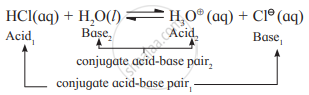
\includegraphics[scale=0.5]{conjugate}
   \end{enumerate}

   \subsection{Label the conjugate acid-base pair in the following reaction:
   \ce{HCl + H2O \rightleftharpoons H3O+ + Cl-}}
   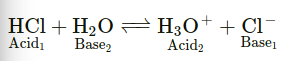
\includegraphics[scale=0.5]{acid-base}

   \section{2-3 M Questions}
   \subsection{Ammonia serves as a Lewis bases whereas $AlCl_3$ is Lewis 
   Acid. Explain}
   \begin{enumerate}
   	\item According to Lewis's theory, an acid is a substance that can 
	accept a share in an electron pair. In the $AlCl_3$ molecule, the 
	octet of $Al$ is incomplete. Therefore, it can accept an electron 
	pair to complete its octet. Hence, $AlCl_3$ acts as a Lewis acid.

	\item According to Lewis theory, a base is a substance that can 
	donate an electron pair. In the ammonia ($NH_3$) molecules, the 
	nitrogen atom has one lone pair of electron to donate. Hence, 
	$NH_3$ acts as Lewis base.
   \end{enumerate}

   

\end{document}
